\documentclass[1p]{elsarticle_modified}
%\bibliographystyle{elsarticle-num}

%\usepackage[colorlinks]{hyperref}
%\usepackage{abbrmath_seonhwa} %\Abb, \Ascr, \Acal ,\Abf, \Afrak
\usepackage{amsfonts}
\usepackage{amssymb}
\usepackage{amsmath}
\usepackage{amsthm}
\usepackage{scalefnt}
\usepackage{amsbsy}
\usepackage{kotex}
\usepackage{caption}
\usepackage{subfig}
\usepackage{color}
\usepackage{graphicx}
\usepackage{xcolor} %% white, black, red, green, blue, cyan, magenta, yellow
\usepackage{float}
\usepackage{setspace}
\usepackage{hyperref}

\usepackage{tikz}
\usetikzlibrary{arrows}

\usepackage{multirow}
\usepackage{array} % fixed length table
\usepackage{hhline}

%%%%%%%%%%%%%%%%%%%%%
\makeatletter
\renewcommand*\env@matrix[1][\arraystretch]{%
	\edef\arraystretch{#1}%
	\hskip -\arraycolsep
	\let\@ifnextchar\new@ifnextchar
	\array{*\c@MaxMatrixCols c}}
\makeatother %https://tex.stackexchange.com/questions/14071/how-can-i-increase-the-line-spacing-in-a-matrix
%%%%%%%%%%%%%%%

\usepackage[normalem]{ulem}

\newcommand{\msout}[1]{\ifmmode\text{\sout{\ensuremath{#1}}}\else\sout{#1}\fi}
%SOURCE: \msout is \stkout macro in https://tex.stackexchange.com/questions/20609/strikeout-in-math-mode

\newcommand{\cancel}[1]{
	\ifmmode
	{\color{red}\msout{#1}}
	\else
	{\color{red}\sout{#1}}
	\fi
}

\newcommand{\add}[1]{
	{\color{blue}\uwave{#1}}
}

\newcommand{\replace}[2]{
	\ifmmode
	{\color{red}\msout{#1}}{\color{blue}\uwave{#2}}
	\else
	{\color{red}\sout{#1}}{\color{blue}\uwave{#2}}
	\fi
}

\newcommand{\Sol}{\mathcal{S}} %segment
\newcommand{\D}{D} %diagram
\newcommand{\A}{\mathcal{A}} %arc


%%%%%%%%%%%%%%%%%%%%%%%%%%%%%5 test

\def\sl{\operatorname{\textup{SL}}(2,\Cbb)}
\def\psl{\operatorname{\textup{PSL}}(2,\Cbb)}
\def\quan{\mkern 1mu \triangleright \mkern 1mu}

\theoremstyle{definition}
\newtheorem{thm}{Theorem}[section]
\newtheorem{prop}[thm]{Proposition}
\newtheorem{lem}[thm]{Lemma}
\newtheorem{ques}[thm]{Question}
\newtheorem{cor}[thm]{Corollary}
\newtheorem{defn}[thm]{Definition}
\newtheorem{exam}[thm]{Example}
\newtheorem{rmk}[thm]{Remark}
\newtheorem{alg}[thm]{Algorithm}

\newcommand{\I}{\sqrt{-1}}
\begin{document}

%\begin{frontmatter}
%
%\title{Boundary parabolic representations of knots up to 8 crossings}
%
%%% Group authors per affiliation:
%\author{Yunhi Cho} 
%\address{Department of Mathematics, University of Seoul, Seoul, Korea}
%\ead{yhcho@uos.ac.kr}
%
%
%\author{Seonhwa Kim} %\fnref{s_kim}}
%\address{Center for Geometry and Physics, Institute for Basic Science, Pohang, 37673, Korea}
%\ead{ryeona17@ibs.re.kr}
%
%\author{Hyuk Kim}
%\address{Department of Mathematical Sciences, Seoul National University, Seoul 08826, Korea}
%\ead{hyukkim@snu.ac.kr}
%
%\author{Seokbeom Yoon}
%\address{Department of Mathematical Sciences, Seoul National University, Seoul, 08826,  Korea}
%\ead{sbyoon15@snu.ac.kr}
%
%\begin{abstract}
%We find all boundary parabolic representation of knots up to 8 crossings.
%
%\end{abstract}
%\begin{keyword}
%    \MSC[2010] 57M25 
%\end{keyword}
%
%\end{frontmatter}

%\linenumbers
%\tableofcontents
%
\newcommand\colored[1]{\textcolor{white}{\rule[-0.35ex]{0.8em}{1.4ex}}\kern-0.8em\color{red} #1}%
%\newcommand\colored[1]{\textcolor{white}{ #1}\kern-2.17ex	\textcolor{white}{ #1}\kern-1.81ex	\textcolor{white}{ #1}\kern-2.15ex\color{red}#1	}

{\Large $\underline{12n_{0667}~(K12n_{0667})}$}

\setlength{\tabcolsep}{10pt}
\renewcommand{\arraystretch}{1.6}
\vspace{1cm}\begin{tabular}{m{100pt}>{\centering\arraybackslash}m{274pt}}
\multirow{5}{120pt}{
	\centering
	\includegraphics[width=112pt]{../../../GIT/diagram.site/Diagrams/png/2756_12n_0667.png}\\
\ \ \ A knot diagram\footnotemark}&
\allowdisplaybreaks
\textbf{Linearized knot diagam} \\
\cline{2-2}
 &
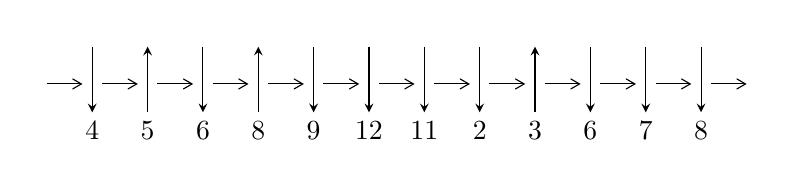
\begin{tikzpicture}[x=20pt, y=17pt]
	% nodes
	\node (C0) at (0, 0) {};
	\node (C1) at (1, 0) {};
	\node (C1U) at (1, +1) {};
	\node (C1D) at (1, -1) {4};

	\node (C2) at (2, 0) {};
	\node (C2U) at (2, +1) {};
	\node (C2D) at (2, -1) {5};

	\node (C3) at (3, 0) {};
	\node (C3U) at (3, +1) {};
	\node (C3D) at (3, -1) {6};

	\node (C4) at (4, 0) {};
	\node (C4U) at (4, +1) {};
	\node (C4D) at (4, -1) {8};

	\node (C5) at (5, 0) {};
	\node (C5U) at (5, +1) {};
	\node (C5D) at (5, -1) {9};

	\node (C6) at (6, 0) {};
	\node (C6U) at (6, +1) {};
	\node (C6D) at (6, -1) {12};

	\node (C7) at (7, 0) {};
	\node (C7U) at (7, +1) {};
	\node (C7D) at (7, -1) {11};

	\node (C8) at (8, 0) {};
	\node (C8U) at (8, +1) {};
	\node (C8D) at (8, -1) {2};

	\node (C9) at (9, 0) {};
	\node (C9U) at (9, +1) {};
	\node (C9D) at (9, -1) {3};

	\node (C10) at (10, 0) {};
	\node (C10U) at (10, +1) {};
	\node (C10D) at (10, -1) {6};

	\node (C11) at (11, 0) {};
	\node (C11U) at (11, +1) {};
	\node (C11D) at (11, -1) {7};

	\node (C12) at (12, 0) {};
	\node (C12U) at (12, +1) {};
	\node (C12D) at (12, -1) {8};
	\node (C13) at (13, 0) {};

	% arrows
	\draw[->,>={angle 60}]
	(C0) edge (C1) (C1) edge (C2) (C2) edge (C3) (C3) edge (C4) (C4) edge (C5) (C5) edge (C6) (C6) edge (C7) (C7) edge (C8) (C8) edge (C9) (C9) edge (C10) (C10) edge (C11) (C11) edge (C12) (C12) edge (C13) ;	\draw[->,>=stealth]
	(C1U) edge (C1D) (C2D) edge (C2U) (C3U) edge (C3D) (C4D) edge (C4U) (C5U) edge (C5D) (C6U) edge (C6D) (C7U) edge (C7D) (C8U) edge (C8D) (C9D) edge (C9U) (C10U) edge (C10D) (C11U) edge (C11D) (C12U) edge (C12D) ;
	\end{tikzpicture} \\
\hhline{~~} \\& 
\textbf{Solving Sequence} \\ \cline{2-2} 
 &
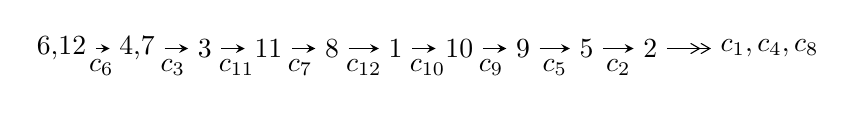
\begin{tikzpicture}[x=23pt, y=7pt]
	% node
	\node (A0) at (-1/8, 0) {6,12};
	\node (A1) at (17/16, 0) {4,7};
	\node (A2) at (17/8, 0) {3};
	\node (A3) at (25/8, 0) {11};
	\node (A4) at (33/8, 0) {8};
	\node (A5) at (41/8, 0) {1};
	\node (A6) at (49/8, 0) {10};
	\node (A7) at (57/8, 0) {9};
	\node (A8) at (65/8, 0) {5};
	\node (A9) at (73/8, 0) {2};
	\node (C1) at (1/2, -1) {$c_{6}$};
	\node (C2) at (13/8, -1) {$c_{3}$};
	\node (C3) at (21/8, -1) {$c_{11}$};
	\node (C4) at (29/8, -1) {$c_{7}$};
	\node (C5) at (37/8, -1) {$c_{12}$};
	\node (C6) at (45/8, -1) {$c_{10}$};
	\node (C7) at (53/8, -1) {$c_{9}$};
	\node (C8) at (61/8, -1) {$c_{5}$};
	\node (C9) at (69/8, -1) {$c_{2}$};
	\node (A10) at (11, 0) {$c_{1},c_{4},c_{8}$};

	% edge
	\draw[->,>=stealth]	
	(A0) edge (A1) (A1) edge (A2) (A2) edge (A3) (A3) edge (A4) (A4) edge (A5) (A5) edge (A6) (A6) edge (A7) (A7) edge (A8) (A8) edge (A9) ;
	\draw[->>,>={angle 60}]	
	(A9) edge (A10);
\end{tikzpicture} \\ 

\end{tabular} \\

\footnotetext{
The image of knot diagram is generated by the software ``\textbf{Draw programme}" developed by Andrew Bartholomew(\url{http://www.layer8.co.uk/maths/draw/index.htm\#Running-draw}), where we modified some parts for our purpose(\url{https://github.com/CATsTAILs/LinksPainter}).
}\phantom \\ \newline 
\centering \textbf{Ideals for irreducible components\footnotemark of $X_{\text{par}}$} 
 
\begin{align*}
I^u_{1}&=\langle 
-3 u^{20}-26 u^{19}+\cdots+7 b+97,\;-83 u^{20}-325 u^{19}+\cdots+63 a+558,\;u^{21}+5 u^{20}+\cdots-72 u-9\rangle \\
I^u_{2}&=\langle 
-3 u^{14} a+5 u^{14}+\cdots+a+24,\;- u^{14} a+2 u^{13} a+\cdots+3 a+4,\;u^{15}-2 u^{14}+\cdots-4 u+1\rangle \\
I^u_{3}&=\langle 
- u^6-2 u^5-5 u^4-6 u^3-6 u^2+b-4 u-1,\;u^8+2 u^7+7 u^6+10 u^5+15 u^4+14 u^3+9 u^2+a+5 u-1,\\
\phantom{I^u_{3}}&\phantom{= \langle  }u^9+2 u^8+7 u^7+10 u^6+16 u^5+16 u^4+13 u^3+9 u^2+2 u+1\rangle \\
I^u_{4}&=\langle 
b+1,\;2 u^2 a+a^2-2 a u+3 a+u-1,\;u^3- u^2+2 u-1\rangle \\
\\
I^v_{1}&=\langle 
a,\;b+1,\;v+1\rangle \\
\end{align*}
\raggedright * 5 irreducible components of $\dim_{\mathbb{C}}=0$, with total 67 representations.\\
\footnotetext{All coefficients of polynomials are rational numbers. But the coefficients are sometimes approximated in decimal forms when there is not enough margin.}
\newpage
\renewcommand{\arraystretch}{1}
\centering \section*{I. $I^u_{1}= \langle -3 u^{20}-26 u^{19}+\cdots+7 b+97,\;-83 u^{20}-325 u^{19}+\cdots+63 a+558,\;u^{21}+5 u^{20}+\cdots-72 u-9 \rangle$}
\flushleft \textbf{(i) Arc colorings}\\
\begin{tabular}{m{7pt} m{180pt} m{7pt} m{180pt} }
\flushright $a_{6}=$&$\begin{pmatrix}1\\0\end{pmatrix}$ \\
\flushright $a_{12}=$&$\begin{pmatrix}0\\u\end{pmatrix}$ \\
\flushright $a_{4}=$&$\begin{pmatrix}\frac{83}{63} u^{20}+\frac{325}{63} u^{19}+\cdots-66 u-\frac{62}{7}\\\frac{3}{7} u^{20}+\frac{26}{7} u^{19}+\cdots-95 u-\frac{97}{7}\end{pmatrix}$ \\
\flushright $a_{7}=$&$\begin{pmatrix}1\\u^2\end{pmatrix}$ \\
\flushright $a_{3}=$&$\begin{pmatrix}\frac{110}{63} u^{20}+\frac{559}{63} u^{19}+\cdots-161 u-\frac{159}{7}\\\frac{3}{7} u^{20}+\frac{26}{7} u^{19}+\cdots-95 u-\frac{97}{7}\end{pmatrix}$ \\
\flushright $a_{11}=$&$\begin{pmatrix}u\\u^3+u\end{pmatrix}$ \\
\flushright $a_{8}=$&$\begin{pmatrix}u^2+1\\u^4+2 u^2\end{pmatrix}$ \\
\flushright $a_{1}=$&$\begin{pmatrix}- u^5-2 u^3- u\\- u^7-3 u^5-2 u^3+u\end{pmatrix}$ \\
\flushright $a_{10}=$&$\begin{pmatrix}u^3+2 u\\u^3+u\end{pmatrix}$ \\
\flushright $a_{9}=$&$\begin{pmatrix}\frac{83}{63} u^{20}+\frac{325}{63} u^{19}+\cdots-86 u-\frac{90}{7}\\\frac{5}{7} u^{20}+\frac{20}{7} u^{19}+\cdots-52 u-\frac{52}{7}\end{pmatrix}$ \\
\flushright $a_{5}=$&$\begin{pmatrix}-\frac{97}{63} u^{20}-\frac{458}{63} u^{19}+\cdots+111 u+\frac{111}{7}\\\frac{1}{7} u^{20}-\frac{10}{7} u^{19}+\cdots+103 u+\frac{110}{7}\end{pmatrix}$ \\
\flushright $a_{2}=$&$\begin{pmatrix}-\frac{52}{63} u^{20}-\frac{215}{63} u^{19}+\cdots+39 u+\frac{38}{7}\\\frac{2}{7} u^{20}+\frac{1}{7} u^{19}+\cdots+36 u+\frac{38}{7}\end{pmatrix}$\\&\end{tabular}
\flushleft \textbf{(ii) Obstruction class $= -1$}\\~\\
\flushleft \textbf{(iii) Cusp Shapes $= \frac{4}{7} u^{20}+\frac{51}{7} u^{19}+\cdots-324 u-\frac{456}{7}$}\\~\\
\newpage\renewcommand{\arraystretch}{1}
\flushleft \textbf{(iv) u-Polynomials at the component}\newline \\
\begin{tabular}{m{50pt}|m{274pt}}
Crossings & \hspace{64pt}u-Polynomials at each crossing \\
\hline $$\begin{aligned}c_{1},c_{3}\end{aligned}$$&$\begin{aligned}
&u^{21}+2 u^{20}+\cdots+8 u+1
\end{aligned}$\\
\hline $$\begin{aligned}c_{2}\end{aligned}$$&$\begin{aligned}
&u^{21}+15 u^{20}+\cdots+63 u+9
\end{aligned}$\\
\hline $$\begin{aligned}c_{4},c_{9}\end{aligned}$$&$\begin{aligned}
&u^{21}-2 u^{20}+\cdots-11 u^2+1
\end{aligned}$\\
\hline $$\begin{aligned}c_{5},c_{8}\end{aligned}$$&$\begin{aligned}
&u^{21}- u^{20}+\cdots- u-1
\end{aligned}$\\
\hline $$\begin{aligned}c_{6},c_{7},c_{11}\end{aligned}$$&$\begin{aligned}
&u^{21}+5 u^{20}+\cdots-72 u-9
\end{aligned}$\\
\hline $$\begin{aligned}c_{10},c_{12}\end{aligned}$$&$\begin{aligned}
&u^{21}-5 u^{20}+\cdots-2988 u-1413
\end{aligned}$\\
\hline
\end{tabular}\\~\\
\newpage\renewcommand{\arraystretch}{1}
\flushleft \textbf{(v) Riley Polynomials at the component}\newline \\
\begin{tabular}{m{50pt}|m{274pt}}
Crossings & \hspace{64pt}Riley Polynomials at each crossing \\
\hline $$\begin{aligned}c_{1},c_{3}\end{aligned}$$&$\begin{aligned}
&y^{21}+30 y^{20}+\cdots+6 y-1
\end{aligned}$\\
\hline $$\begin{aligned}c_{2}\end{aligned}$$&$\begin{aligned}
&y^{21}-13 y^{20}+\cdots-1377 y-81
\end{aligned}$\\
\hline $$\begin{aligned}c_{4},c_{9}\end{aligned}$$&$\begin{aligned}
&y^{21}-22 y^{20}+\cdots+22 y-1
\end{aligned}$\\
\hline $$\begin{aligned}c_{5},c_{8}\end{aligned}$$&$\begin{aligned}
&y^{21}-11 y^{20}+\cdots+21 y-1
\end{aligned}$\\
\hline $$\begin{aligned}c_{6},c_{7},c_{11}\end{aligned}$$&$\begin{aligned}
&y^{21}+23 y^{20}+\cdots+324 y-81
\end{aligned}$\\
\hline $$\begin{aligned}c_{10},c_{12}\end{aligned}$$&$\begin{aligned}
&y^{21}+19 y^{20}+\cdots-3839724 y-1996569
\end{aligned}$\\
\hline
\end{tabular}\\~\\
\newpage\flushleft \textbf{(vi) Complex Volumes and Cusp Shapes}
$$\begin{array}{c|c|c}  
\text{Solutions to }I^u_{1}& \I (\text{vol} + \sqrt{-1}CS) & \text{Cusp shape}\\
 \hline 
\begin{aligned}
u &= -0.834623 + 0.573705 I \\
a &= \phantom{-}1.005930 + 0.264258 I \\
b &= \phantom{-}0.62121 - 1.82385 I\end{aligned}
 & \phantom{-}6.40877 + 10.26430 I & -4.52348 - 6.93928 I \\ \hline\begin{aligned}
u &= -0.834623 - 0.573705 I \\
a &= \phantom{-}1.005930 - 0.264258 I \\
b &= \phantom{-}0.62121 + 1.82385 I\end{aligned}
 & \phantom{-}6.40877 - 10.26430 I & -4.52348 + 6.93928 I \\ \hline\begin{aligned}
u &= -0.847213 + 0.586710 I \\
a &= -0.922945 + 0.173773 I \\
b &= \phantom{-}0.16137 + 1.79856 I\end{aligned}
 & \phantom{-}6.42391 - 4.68256 I & -3.99466 + 2.17560 I \\ \hline\begin{aligned}
u &= -0.847213 - 0.586710 I \\
a &= -0.922945 - 0.173773 I \\
b &= \phantom{-}0.16137 - 1.79856 I\end{aligned}
 & \phantom{-}6.42391 + 4.68256 I & -3.99466 - 2.17560 I \\ \hline\begin{aligned}
u &= \phantom{-}0.825151\phantom{ +0.000000I} \\
a &= -0.722716\phantom{ +0.000000I} \\
b &= -0.926404\phantom{ +0.000000I}\end{aligned}
 & -5.68389\phantom{ +0.000000I} & -17.0230\phantom{ +0.000000I} \\ \hline\begin{aligned}
u &= -0.150569 + 1.281090 I \\
a &= \phantom{-}0.434742 - 0.402686 I \\
b &= \phantom{-}0.074569 + 0.138439 I\end{aligned}
 & \phantom{-}3.22602 + 2.41816 I & -3.53897 - 1.93549 I \\ \hline\begin{aligned}
u &= -0.150569 - 1.281090 I \\
a &= \phantom{-}0.434742 + 0.402686 I \\
b &= \phantom{-}0.074569 - 0.138439 I\end{aligned}
 & \phantom{-}3.22602 - 2.41816 I & -3.53897 + 1.93549 I \\ \hline\begin{aligned}
u &= -0.323088 + 0.617615 I \\
a &= \phantom{-}0.358624 - 0.512504 I \\
b &= -0.096498 + 0.850760 I\end{aligned}
 & \phantom{-}0.52795 + 2.17494 I & -5.93194 - 4.33334 I \\ \hline\begin{aligned}
u &= -0.323088 - 0.617615 I \\
a &= \phantom{-}0.358624 + 0.512504 I \\
b &= -0.096498 - 0.850760 I\end{aligned}
 & \phantom{-}0.52795 - 2.17494 I & -5.93194 + 4.33334 I \\ \hline\begin{aligned}
u &= \phantom{-}0.373837 + 1.314800 I \\
a &= \phantom{-}0.363936 + 0.564961 I \\
b &= -0.998750 + 0.204857 I\end{aligned}
 & -1.57111 - 4.30895 I & -11.00324 + 1.55396 I\\
 \hline 
 \end{array}$$\newpage$$\begin{array}{c|c|c}  
\text{Solutions to }I^u_{1}& \I (\text{vol} + \sqrt{-1}CS) & \text{Cusp shape}\\
 \hline 
\begin{aligned}
u &= \phantom{-}0.373837 - 1.314800 I \\
a &= \phantom{-}0.363936 - 0.564961 I \\
b &= -0.998750 - 0.204857 I\end{aligned}
 & -1.57111 + 4.30895 I & -11.00324 - 1.55396 I \\ \hline\begin{aligned}
u &= -0.027283 + 1.412760 I \\
a &= \phantom{-}0.78061 + 1.55576 I \\
b &= -1.109230 - 0.677694 I\end{aligned}
 & \phantom{-}3.18953 + 0.20531 I & -5.89178 + 0.57061 I \\ \hline\begin{aligned}
u &= -0.027283 - 1.412760 I \\
a &= \phantom{-}0.78061 - 1.55576 I \\
b &= -1.109230 + 0.677694 I\end{aligned}
 & \phantom{-}3.18953 - 0.20531 I & -5.89178 - 0.57061 I \\ \hline\begin{aligned}
u &= -0.437416 + 0.103332 I \\
a &= \phantom{-}0.929988 - 0.551312 I \\
b &= -0.189823 + 0.028334 I\end{aligned}
 & -0.974855 + 0.275619 I & -10.86571 - 2.54923 I \\ \hline\begin{aligned}
u &= -0.437416 - 0.103332 I \\
a &= \phantom{-}0.929988 + 0.551312 I \\
b &= -0.189823 - 0.028334 I\end{aligned}
 & -0.974855 - 0.275619 I & -10.86571 + 2.54923 I \\ \hline\begin{aligned}
u &= -0.09149 + 1.57120 I \\
a &= -0.26719 - 1.73552 I \\
b &= \phantom{-}0.33826 + 1.86261 I\end{aligned}
 & \phantom{-}7.94844 + 3.68537 I & -6.18348 + 2.45338 I \\ \hline\begin{aligned}
u &= -0.09149 - 1.57120 I \\
a &= -0.26719 + 1.73552 I \\
b &= \phantom{-}0.33826 - 1.86261 I\end{aligned}
 & \phantom{-}7.94844 - 3.68537 I & -6.18348 - 2.45338 I \\ \hline\begin{aligned}
u &= -0.28888 + 1.56597 I \\
a &= \phantom{-}0.45254 + 2.00394 I \\
b &= \phantom{-}1.01317 - 2.01561 I\end{aligned}
 & \phantom{-}13.4087 + 14.4061 I & -2.12525 - 6.98840 I \\ \hline\begin{aligned}
u &= -0.28888 - 1.56597 I \\
a &= \phantom{-}0.45254 - 2.00394 I \\
b &= \phantom{-}1.01317 + 2.01561 I\end{aligned}
 & \phantom{-}13.4087 - 14.4061 I & -2.12525 + 6.98840 I \\ \hline\begin{aligned}
u &= -0.28585 + 1.59217 I \\
a &= -0.77487 - 1.52631 I \\
b &= -0.35107 + 2.01142 I\end{aligned}
 & \phantom{-}13.60260 - 0.45994 I & -1.43013 + 1.46856 I\\
 \hline 
 \end{array}$$\newpage$$\begin{array}{c|c|c}  
\text{Solutions to }I^u_{1}& \I (\text{vol} + \sqrt{-1}CS) & \text{Cusp shape}\\
 \hline 
\begin{aligned}
u &= -0.28585 - 1.59217 I \\
a &= -0.77487 + 1.52631 I \\
b &= -0.35107 - 2.01142 I\end{aligned}
 & \phantom{-}13.60260 + 0.45994 I & -1.43013 - 1.46856 I\\
 \hline 
 \end{array}$$\newpage\newpage\renewcommand{\arraystretch}{1}
\centering \section*{II. $I^u_{2}= \langle -3 u^{14} a+5 u^{14}+\cdots+a+24,\;- u^{14} a+2 u^{13} a+\cdots+3 a+4,\;u^{15}-2 u^{14}+\cdots-4 u+1 \rangle$}
\flushleft \textbf{(i) Arc colorings}\\
\begin{tabular}{m{7pt} m{180pt} m{7pt} m{180pt} }
\flushright $a_{6}=$&$\begin{pmatrix}1\\0\end{pmatrix}$ \\
\flushright $a_{12}=$&$\begin{pmatrix}0\\u\end{pmatrix}$ \\
\flushright $a_{4}=$&$\begin{pmatrix}a\\\frac{3}{14} u^{14} a-\frac{5}{14} u^{14}+\cdots-\frac{1}{14} a-\frac{12}{7}\end{pmatrix}$ \\
\flushright $a_{7}=$&$\begin{pmatrix}1\\u^2\end{pmatrix}$ \\
\flushright $a_{3}=$&$\begin{pmatrix}0.214286 a u^{14}-0.357143 u^{14}+\cdots+0.928571 a-1.71429\\\frac{3}{14} u^{14} a-\frac{5}{14} u^{14}+\cdots-\frac{1}{14} a-\frac{12}{7}\end{pmatrix}$ \\
\flushright $a_{11}=$&$\begin{pmatrix}u\\u^3+u\end{pmatrix}$ \\
\flushright $a_{8}=$&$\begin{pmatrix}u^2+1\\u^4+2 u^2\end{pmatrix}$ \\
\flushright $a_{1}=$&$\begin{pmatrix}- u^5-2 u^3- u\\- u^7-3 u^5-2 u^3+u\end{pmatrix}$ \\
\flushright $a_{10}=$&$\begin{pmatrix}u^3+2 u\\u^3+u\end{pmatrix}$ \\
\flushright $a_{9}=$&$\begin{pmatrix}\frac{10}{7} u^{14} a+\frac{9}{7} u^{14}+\cdots-\frac{8}{7} a-\frac{10}{7}\\\frac{5}{14} u^{14} a+\frac{1}{14} u^{14}+\cdots-\frac{25}{14} a-\frac{6}{7}\end{pmatrix}$ \\
\flushright $a_{5}=$&$\begin{pmatrix}-\frac{1}{14} u^{14} a-\frac{5}{7} u^{14}+\cdots+\frac{6}{7} a+\frac{1}{14}\\-0.142857 a u^{14}-0.928571 u^{14}+\cdots+0.214286 a-0.357143\end{pmatrix}$ \\
\flushright $a_{2}=$&$\begin{pmatrix}\frac{5}{14} u^{14} a-\frac{3}{7} u^{14}+\cdots+\frac{12}{7} a+\frac{9}{14}\\1\end{pmatrix}$\\&\end{tabular}
\flushleft \textbf{(ii) Obstruction class $= -1$}\\~\\
\flushleft \textbf{(iii) Cusp Shapes $= 11 u^{14}-16 u^{13}+97 u^{12}-120 u^{11}+326 u^{10}-337 u^9+511 u^8-400 u^7+342 u^6-95 u^5+10 u^4+150 u^3-84 u^2+55 u-19$}\\~\\
\newpage\renewcommand{\arraystretch}{1}
\flushleft \textbf{(iv) u-Polynomials at the component}\newline \\
\begin{tabular}{m{50pt}|m{274pt}}
Crossings & \hspace{64pt}u-Polynomials at each crossing \\
\hline $$\begin{aligned}c_{1},c_{3}\end{aligned}$$&$\begin{aligned}
&u^{30}-7 u^{29}+\cdots-676 u-329
\end{aligned}$\\
\hline $$\begin{aligned}c_{2}\end{aligned}$$&$\begin{aligned}
&(u^{15}-7 u^{14}+\cdots+28 u-8)^{2}
\end{aligned}$\\
\hline $$\begin{aligned}c_{4},c_{9}\end{aligned}$$&$\begin{aligned}
&u^{30}-14 u^{28}+\cdots-641 u+151
\end{aligned}$\\
\hline $$\begin{aligned}c_{5},c_{8}\end{aligned}$$&$\begin{aligned}
&u^{30}+9 u^{26}+\cdots- u-1
\end{aligned}$\\
\hline $$\begin{aligned}c_{6},c_{7},c_{11}\end{aligned}$$&$\begin{aligned}
&(u^{15}-2 u^{14}+\cdots-4 u+1)^{2}
\end{aligned}$\\
\hline $$\begin{aligned}c_{10},c_{12}\end{aligned}$$&$\begin{aligned}
&(u^{15}+2 u^{14}+\cdots-16 u+5)^{2}
\end{aligned}$\\
\hline
\end{tabular}\\~\\
\newpage\renewcommand{\arraystretch}{1}
\flushleft \textbf{(v) Riley Polynomials at the component}\newline \\
\begin{tabular}{m{50pt}|m{274pt}}
Crossings & \hspace{64pt}Riley Polynomials at each crossing \\
\hline $$\begin{aligned}c_{1},c_{3}\end{aligned}$$&$\begin{aligned}
&y^{30}+33 y^{29}+\cdots+1028130 y+108241
\end{aligned}$\\
\hline $$\begin{aligned}c_{2}\end{aligned}$$&$\begin{aligned}
&(y^{15}-7 y^{14}+\cdots+528 y-64)^{2}
\end{aligned}$\\
\hline $$\begin{aligned}c_{4},c_{9}\end{aligned}$$&$\begin{aligned}
&y^{30}-28 y^{29}+\cdots+125773 y+22801
\end{aligned}$\\
\hline $$\begin{aligned}c_{5},c_{8}\end{aligned}$$&$\begin{aligned}
&y^{30}+18 y^{28}+\cdots-35 y+1
\end{aligned}$\\
\hline $$\begin{aligned}c_{6},c_{7},c_{11}\end{aligned}$$&$\begin{aligned}
&(y^{15}+16 y^{14}+\cdots-4 y-1)^{2}
\end{aligned}$\\
\hline $$\begin{aligned}c_{10},c_{12}\end{aligned}$$&$\begin{aligned}
&(y^{15}+16 y^{14}+\cdots-344 y-25)^{2}
\end{aligned}$\\
\hline
\end{tabular}\\~\\
\newpage\flushleft \textbf{(vi) Complex Volumes and Cusp Shapes}
$$\begin{array}{c|c|c}  
\text{Solutions to }I^u_{2}& \I (\text{vol} + \sqrt{-1}CS) & \text{Cusp shape}\\
 \hline 
\begin{aligned}
u &= \phantom{-}0.783022 + 0.548748 I \\
a &= -0.815000 - 0.070479 I \\
b &= \phantom{-}0.23196 - 1.72434 I\end{aligned}
 & \phantom{-}7.57107 - 2.60312 I & -2.84235 + 2.92184 I \\ \hline\begin{aligned}
u &= \phantom{-}0.783022 + 0.548748 I \\
a &= \phantom{-}1.150630 - 0.405666 I \\
b &= \phantom{-}0.61243 + 1.61879 I\end{aligned}
 & \phantom{-}7.57107 - 2.60312 I & -2.84235 + 2.92184 I \\ \hline\begin{aligned}
u &= \phantom{-}0.783022 - 0.548748 I \\
a &= -0.815000 + 0.070479 I \\
b &= \phantom{-}0.23196 + 1.72434 I\end{aligned}
 & \phantom{-}7.57107 + 2.60312 I & -2.84235 - 2.92184 I \\ \hline\begin{aligned}
u &= \phantom{-}0.783022 - 0.548748 I \\
a &= \phantom{-}1.150630 + 0.405666 I \\
b &= \phantom{-}0.61243 - 1.61879 I\end{aligned}
 & \phantom{-}7.57107 + 2.60312 I & -2.84235 - 2.92184 I \\ \hline\begin{aligned}
u &= -0.216855 + 1.221530 I \\
a &= \phantom{-}0.741221 - 0.405618 I \\
b &= -0.661072 + 0.460812 I\end{aligned}
 & \phantom{-}1.58567 + 3.38986 I & -3.26125 - 8.75376 I \\ \hline\begin{aligned}
u &= -0.216855 + 1.221530 I \\
a &= \phantom{-}0.660981 + 1.010040 I \\
b &= \phantom{-}0.913612 + 0.021844 I\end{aligned}
 & \phantom{-}1.58567 + 3.38986 I & -3.26125 - 8.75376 I \\ \hline\begin{aligned}
u &= -0.216855 - 1.221530 I \\
a &= \phantom{-}0.741221 + 0.405618 I \\
b &= -0.661072 - 0.460812 I\end{aligned}
 & \phantom{-}1.58567 - 3.38986 I & -3.26125 + 8.75376 I \\ \hline\begin{aligned}
u &= -0.216855 - 1.221530 I \\
a &= \phantom{-}0.660981 - 1.010040 I \\
b &= \phantom{-}0.913612 - 0.021844 I\end{aligned}
 & \phantom{-}1.58567 - 3.38986 I & -3.26125 + 8.75376 I \\ \hline\begin{aligned}
u &= -0.699136\phantom{ +0.000000I} \\
a &= \phantom{-}0.498930\phantom{ +0.000000I} \\
b &= -0.445090\phantom{ +0.000000I}\end{aligned}
 & -2.08475\phantom{ +0.000000I} & -3.31340\phantom{ +0.000000I} \\ \hline\begin{aligned}
u &= -0.699136\phantom{ +0.000000I} \\
a &= \phantom{-}1.87307\phantom{ +0.000000I} \\
b &= \phantom{-}0.972659\phantom{ +0.000000I}\end{aligned}
 & -2.08475\phantom{ +0.000000I} & -3.31340\phantom{ +0.000000I}\\
 \hline 
 \end{array}$$\newpage$$\begin{array}{c|c|c}  
\text{Solutions to }I^u_{2}& \I (\text{vol} + \sqrt{-1}CS) & \text{Cusp shape}\\
 \hline 
\begin{aligned}
u &= \phantom{-}0.061637 + 0.608365 I \\
a &= \phantom{-}0.934694 + 0.293027 I \\
b &= \phantom{-}0.986562 + 0.556921 I\end{aligned}
 & \phantom{-}1.61379 + 2.57496 I & -1.10179 - 1.01110 I \\ \hline\begin{aligned}
u &= \phantom{-}0.061637 + 0.608365 I \\
a &= \phantom{-}0.94855 - 1.35297 I \\
b &= -0.329324 + 1.042070 I\end{aligned}
 & \phantom{-}1.61379 + 2.57496 I & -1.10179 - 1.01110 I \\ \hline\begin{aligned}
u &= \phantom{-}0.061637 - 0.608365 I \\
a &= \phantom{-}0.934694 - 0.293027 I \\
b &= \phantom{-}0.986562 - 0.556921 I\end{aligned}
 & \phantom{-}1.61379 - 2.57496 I & -1.10179 + 1.01110 I \\ \hline\begin{aligned}
u &= \phantom{-}0.061637 - 0.608365 I \\
a &= \phantom{-}0.94855 + 1.35297 I \\
b &= -0.329324 - 1.042070 I\end{aligned}
 & \phantom{-}1.61379 - 2.57496 I & -1.10179 + 1.01110 I \\ \hline\begin{aligned}
u &= \phantom{-}0.09920 + 1.46553 I \\
a &= -0.395823 - 0.646191 I \\
b &= -0.609648 + 0.043969 I\end{aligned}
 & \phantom{-}6.22877 - 5.97807 I & -2.99155 + 7.20850 I \\ \hline\begin{aligned}
u &= \phantom{-}0.09920 + 1.46553 I \\
a &= -0.26994 + 2.77190 I \\
b &= -0.31360 - 2.40695 I\end{aligned}
 & \phantom{-}6.22877 - 5.97807 I & -2.99155 + 7.20850 I \\ \hline\begin{aligned}
u &= \phantom{-}0.09920 - 1.46553 I \\
a &= -0.395823 + 0.646191 I \\
b &= -0.609648 - 0.043969 I\end{aligned}
 & \phantom{-}6.22877 + 5.97807 I & -2.99155 - 7.20850 I \\ \hline\begin{aligned}
u &= \phantom{-}0.09920 - 1.46553 I \\
a &= -0.26994 - 2.77190 I \\
b &= -0.31360 + 2.40695 I\end{aligned}
 & \phantom{-}6.22877 + 5.97807 I & -2.99155 - 7.20850 I \\ \hline\begin{aligned}
u &= -0.01760 + 1.52899 I \\
a &= -1.250130 - 0.500701 I \\
b &= \phantom{-}2.00715 + 0.63605 I\end{aligned}
 & \phantom{-}8.69622 + 2.65996 I & \phantom{-}1.50438 - 2.01476 I \\ \hline\begin{aligned}
u &= -0.01760 + 1.52899 I \\
a &= \phantom{-}0.23286 - 2.06811 I \\
b &= -0.18397 + 1.61289 I\end{aligned}
 & \phantom{-}8.69622 + 2.65996 I & \phantom{-}1.50438 - 2.01476 I\\
 \hline 
 \end{array}$$\newpage$$\begin{array}{c|c|c}  
\text{Solutions to }I^u_{2}& \I (\text{vol} + \sqrt{-1}CS) & \text{Cusp shape}\\
 \hline 
\begin{aligned}
u &= -0.01760 - 1.52899 I \\
a &= -1.250130 + 0.500701 I \\
b &= \phantom{-}2.00715 - 0.63605 I\end{aligned}
 & \phantom{-}8.69622 - 2.65996 I & \phantom{-}1.50438 + 2.01476 I \\ \hline\begin{aligned}
u &= -0.01760 - 1.52899 I \\
a &= \phantom{-}0.23286 + 2.06811 I \\
b &= -0.18397 - 1.61289 I\end{aligned}
 & \phantom{-}8.69622 - 2.65996 I & \phantom{-}1.50438 + 2.01476 I \\ \hline\begin{aligned}
u &= \phantom{-}0.367791 + 0.287869 I \\
a &= -1.078570 + 0.747772 I \\
b &= -0.34613 - 1.55473 I\end{aligned}
 & \phantom{-}0.39798 - 4.38767 I & -9.5578 + 11.0682 I \\ \hline\begin{aligned}
u &= \phantom{-}0.367791 + 0.287869 I \\
a &= -1.52156 - 2.49296 I \\
b &= -0.006820 - 0.312135 I\end{aligned}
 & \phantom{-}0.39798 - 4.38767 I & -9.5578 + 11.0682 I \\ \hline\begin{aligned}
u &= \phantom{-}0.367791 - 0.287869 I \\
a &= -1.078570 - 0.747772 I \\
b &= -0.34613 + 1.55473 I\end{aligned}
 & \phantom{-}0.39798 + 4.38767 I & -9.5578 - 11.0682 I \\ \hline\begin{aligned}
u &= \phantom{-}0.367791 - 0.287869 I \\
a &= -1.52156 + 2.49296 I \\
b &= -0.006820 + 0.312135 I\end{aligned}
 & \phantom{-}0.39798 + 4.38767 I & -9.5578 - 11.0682 I \\ \hline\begin{aligned}
u &= \phantom{-}0.27238 + 1.54795 I \\
a &= -0.97464 + 1.65279 I \\
b &= -0.05742 - 2.01595 I\end{aligned}
 & \phantom{-}14.4273 - 6.4879 I & -0.59296 + 3.62205 I \\ \hline\begin{aligned}
u &= \phantom{-}0.27238 + 1.54795 I \\
a &= \phantom{-}0.45074 - 1.92343 I \\
b &= \phantom{-}0.99248 + 1.70658 I\end{aligned}
 & \phantom{-}14.4273 - 6.4879 I & -0.59296 + 3.62205 I \\ \hline\begin{aligned}
u &= \phantom{-}0.27238 - 1.54795 I \\
a &= -0.97464 - 1.65279 I \\
b &= -0.05742 + 2.01595 I\end{aligned}
 & \phantom{-}14.4273 + 6.4879 I & -0.59296 - 3.62205 I \\ \hline\begin{aligned}
u &= \phantom{-}0.27238 - 1.54795 I \\
a &= \phantom{-}0.45074 + 1.92343 I \\
b &= \phantom{-}0.99248 - 1.70658 I\end{aligned}
 & \phantom{-}14.4273 + 6.4879 I & -0.59296 - 3.62205 I\\
 \hline 
 \end{array}$$\newpage\newpage\renewcommand{\arraystretch}{1}
\centering \section*{III. $I^u_{3}= \langle - u^6-2 u^5-5 u^4-6 u^3-6 u^2+b-4 u-1,\;u^8+2 u^7+\cdots+a-1,\;u^9+2 u^8+\cdots+2 u+1 \rangle$}
\flushleft \textbf{(i) Arc colorings}\\
\begin{tabular}{m{7pt} m{180pt} m{7pt} m{180pt} }
\flushright $a_{6}=$&$\begin{pmatrix}1\\0\end{pmatrix}$ \\
\flushright $a_{12}=$&$\begin{pmatrix}0\\u\end{pmatrix}$ \\
\flushright $a_{4}=$&$\begin{pmatrix}- u^8-2 u^7-7 u^6-10 u^5-15 u^4-14 u^3-9 u^2-5 u+1\\u^6+2 u^5+5 u^4+6 u^3+6 u^2+4 u+1\end{pmatrix}$ \\
\flushright $a_{7}=$&$\begin{pmatrix}1\\u^2\end{pmatrix}$ \\
\flushright $a_{3}=$&$\begin{pmatrix}- u^8-2 u^7-6 u^6-8 u^5-10 u^4-8 u^3-3 u^2- u+2\\u^6+2 u^5+5 u^4+6 u^3+6 u^2+4 u+1\end{pmatrix}$ \\
\flushright $a_{11}=$&$\begin{pmatrix}u\\u^3+u\end{pmatrix}$ \\
\flushright $a_{8}=$&$\begin{pmatrix}u^2+1\\u^4+2 u^2\end{pmatrix}$ \\
\flushright $a_{1}=$&$\begin{pmatrix}- u^5-2 u^3- u\\- u^7-3 u^5-2 u^3+u\end{pmatrix}$ \\
\flushright $a_{10}=$&$\begin{pmatrix}u^3+2 u\\u^3+u\end{pmatrix}$ \\
\flushright $a_{9}=$&$\begin{pmatrix}- u^7-2 u^6-6 u^5-8 u^4-10 u^3-9 u^2-4 u-3\\- u^8-2 u^7-6 u^6-8 u^5-11 u^4-9 u^3-6 u^2-3 u\end{pmatrix}$ \\
\flushright $a_{5}=$&$\begin{pmatrix}- u^8-2 u^7-7 u^6-9 u^5-14 u^4-11 u^3-7 u^2-3 u+2\\u^7+2 u^6+6 u^5+8 u^4+10 u^3+8 u^2+4 u+1\end{pmatrix}$ \\
\flushright $a_{2}=$&$\begin{pmatrix}- u^8-2 u^7-6 u^6-10 u^5-13 u^4-16 u^3-11 u^2-9 u-3\\- u^7- u^6-4 u^5-3 u^4-4 u^3-2 u^2+1\end{pmatrix}$\\&\end{tabular}
\flushleft \textbf{(ii) Obstruction class $= 1$}\\~\\
\flushleft \textbf{(iii) Cusp Shapes $= u^8-4 u^6-13 u^5-32 u^4-38 u^3-40 u^2-24 u-8$}\\~\\
\newpage\renewcommand{\arraystretch}{1}
\flushleft \textbf{(iv) u-Polynomials at the component}\newline \\
\begin{tabular}{m{50pt}|m{274pt}}
Crossings & \hspace{64pt}u-Polynomials at each crossing \\
\hline $$\begin{aligned}c_{1},c_{3}\end{aligned}$$&$\begin{aligned}
&u^9+3 u^8+9 u^7+14 u^6+18 u^5+18 u^4+13 u^3+8 u^2+4 u+1
\end{aligned}$\\
\hline $$\begin{aligned}c_{2}\end{aligned}$$&$\begin{aligned}
&u^9+12 u^8+\cdots+401 u+89
\end{aligned}$\\
\hline $$\begin{aligned}c_{4},c_{9}\end{aligned}$$&$\begin{aligned}
&u^9- u^8- u^7+2 u^6+2 u^5-2 u^4- u^3+2 u^2-1
\end{aligned}$\\
\hline $$\begin{aligned}c_{5},c_{8}\end{aligned}$$&$\begin{aligned}
&u^9-2 u^7- u^6+2 u^5+2 u^4-2 u^3- u^2+u+1
\end{aligned}$\\
\hline $$\begin{aligned}c_{6},c_{7}\end{aligned}$$&$\begin{aligned}
&u^9+2 u^8+7 u^7+10 u^6+16 u^5+16 u^4+13 u^3+9 u^2+2 u+1
\end{aligned}$\\
\hline $$\begin{aligned}c_{10},c_{12}\end{aligned}$$&$\begin{aligned}
&u^9+2 u^8+3 u^7+u^6-18 u^5-20 u^4-4 u^3-11 u^2-1
\end{aligned}$\\
\hline $$\begin{aligned}c_{11}\end{aligned}$$&$\begin{aligned}
&u^9-2 u^8+7 u^7-10 u^6+16 u^5-16 u^4+13 u^3-9 u^2+2 u-1
\end{aligned}$\\
\hline
\end{tabular}\\~\\
\newpage\renewcommand{\arraystretch}{1}
\flushleft \textbf{(v) Riley Polynomials at the component}\newline \\
\begin{tabular}{m{50pt}|m{274pt}}
Crossings & \hspace{64pt}Riley Polynomials at each crossing \\
\hline $$\begin{aligned}c_{1},c_{3}\end{aligned}$$&$\begin{aligned}
&y^9+9 y^8+33 y^7+46 y^6+14 y^5-14 y^4-3 y^3+4 y^2-1
\end{aligned}$\\
\hline $$\begin{aligned}c_{2}\end{aligned}$$&$\begin{aligned}
&y^9-6 y^8+\cdots+8789 y-7921
\end{aligned}$\\
\hline $$\begin{aligned}c_{4},c_{9}\end{aligned}$$&$\begin{aligned}
&y^9-3 y^8+9 y^7-14 y^6+18 y^5-18 y^4+13 y^3-8 y^2+4 y-1
\end{aligned}$\\
\hline $$\begin{aligned}c_{5},c_{8}\end{aligned}$$&$\begin{aligned}
&y^9-4 y^8+8 y^7-13 y^6+18 y^5-18 y^4+14 y^3-9 y^2+3 y-1
\end{aligned}$\\
\hline $$\begin{aligned}c_{6},c_{7},c_{11}\end{aligned}$$&$\begin{aligned}
&y^9+10 y^8+41 y^7+86 y^6+86 y^5+4 y^4-75 y^3-61 y^2-14 y-1
\end{aligned}$\\
\hline $$\begin{aligned}c_{10},c_{12}\end{aligned}$$&$\begin{aligned}
&y^9+2 y^8-31 y^7-37 y^6+384 y^5-230 y^4-422 y^3-161 y^2-22 y-1
\end{aligned}$\\
\hline
\end{tabular}\\~\\
\newpage\flushleft \textbf{(vi) Complex Volumes and Cusp Shapes}
$$\begin{array}{c|c|c}  
\text{Solutions to }I^u_{3}& \I (\text{vol} + \sqrt{-1}CS) & \text{Cusp shape}\\
 \hline 
\begin{aligned}
u &= -0.942156\phantom{ +0.000000I} \\
a &= \phantom{-}0.835924\phantom{ +0.000000I} \\
b &= \phantom{-}0.693833\phantom{ +0.000000I}\end{aligned}
 & -4.78668\phantom{ +0.000000I} & -6.85480\phantom{ +0.000000I} \\ \hline\begin{aligned}
u &= \phantom{-}0.025437 + 1.219490 I \\
a &= -0.848257 + 0.499627 I \\
b &= -0.174357 - 0.757557 I\end{aligned}
 & \phantom{-}3.87432 - 3.77454 I & -1.17699 + 5.61151 I \\ \hline\begin{aligned}
u &= \phantom{-}0.025437 - 1.219490 I \\
a &= -0.848257 - 0.499627 I \\
b &= -0.174357 + 0.757557 I\end{aligned}
 & \phantom{-}3.87432 + 3.77454 I & -1.17699 - 5.61151 I \\ \hline\begin{aligned}
u &= -0.465053 + 1.257920 I \\
a &= \phantom{-}0.128314 + 0.500319 I \\
b &= \phantom{-}0.628101 + 0.278164 I\end{aligned}
 & -0.89563 + 5.00672 I & -5.11040 - 6.89072 I \\ \hline\begin{aligned}
u &= -0.465053 - 1.257920 I \\
a &= \phantom{-}0.128314 - 0.500319 I \\
b &= \phantom{-}0.628101 - 0.278164 I\end{aligned}
 & -0.89563 - 5.00672 I & -5.11040 + 6.89072 I \\ \hline\begin{aligned}
u &= -0.05596 + 1.56008 I \\
a &= -0.27494 - 1.81410 I \\
b &= \phantom{-}0.58625 + 1.89814 I\end{aligned}
 & \phantom{-}8.14041 + 4.21823 I & -1.16365 - 10.14642 I \\ \hline\begin{aligned}
u &= -0.05596 - 1.56008 I \\
a &= -0.27494 + 1.81410 I \\
b &= \phantom{-}0.58625 - 1.89814 I\end{aligned}
 & \phantom{-}8.14041 - 4.21823 I & -1.16365 + 10.14642 I \\ \hline\begin{aligned}
u &= -0.033345 + 0.402052 I \\
a &= \phantom{-}2.07693 - 1.08799 I \\
b &= \phantom{-}0.113094 + 1.126000 I\end{aligned}
 & \phantom{-}1.14384 + 3.68908 I & -2.12153 - 6.55211 I \\ \hline\begin{aligned}
u &= -0.033345 - 0.402052 I \\
a &= \phantom{-}2.07693 + 1.08799 I \\
b &= \phantom{-}0.113094 - 1.126000 I\end{aligned}
 & \phantom{-}1.14384 - 3.68908 I & -2.12153 + 6.55211 I\\
 \hline 
 \end{array}$$\newpage\newpage\renewcommand{\arraystretch}{1}
\centering \section*{IV. $I^u_{4}= \langle b+1,\;2 u^2 a+a^2-2 a u+3 a+u-1,\;u^3- u^2+2 u-1 \rangle$}
\flushleft \textbf{(i) Arc colorings}\\
\begin{tabular}{m{7pt} m{180pt} m{7pt} m{180pt} }
\flushright $a_{6}=$&$\begin{pmatrix}1\\0\end{pmatrix}$ \\
\flushright $a_{12}=$&$\begin{pmatrix}0\\u\end{pmatrix}$ \\
\flushright $a_{4}=$&$\begin{pmatrix}a\\-1\end{pmatrix}$ \\
\flushright $a_{7}=$&$\begin{pmatrix}1\\u^2\end{pmatrix}$ \\
\flushright $a_{3}=$&$\begin{pmatrix}a-1\\-1\end{pmatrix}$ \\
\flushright $a_{11}=$&$\begin{pmatrix}u\\u^2- u+1\end{pmatrix}$ \\
\flushright $a_{8}=$&$\begin{pmatrix}u^2+1\\u^2- u+1\end{pmatrix}$ \\
\flushright $a_{1}=$&$\begin{pmatrix}-1\\0\end{pmatrix}$ \\
\flushright $a_{10}=$&$\begin{pmatrix}u^2+1\\u^2- u+1\end{pmatrix}$ \\
\flushright $a_{9}=$&$\begin{pmatrix}2 u^2 a- a u+2 a+u+1\\u^2 a- a u+u^2+a+1\end{pmatrix}$ \\
\flushright $a_{5}=$&$\begin{pmatrix}- u^2+u-2\\- a u-2\end{pmatrix}$ \\
\flushright $a_{2}=$&$\begin{pmatrix}a-1\\-1\end{pmatrix}$\\&\end{tabular}
\flushleft \textbf{(ii) Obstruction class $= 1$}\\~\\
\flushleft \textbf{(iii) Cusp Shapes $= -5 u^2-16$}\\~\\
\newpage\renewcommand{\arraystretch}{1}
\flushleft \textbf{(iv) u-Polynomials at the component}\newline \\
\begin{tabular}{m{50pt}|m{274pt}}
Crossings & \hspace{64pt}u-Polynomials at each crossing \\
\hline $$\begin{aligned}c_{1},c_{3}\end{aligned}$$&$\begin{aligned}
&(u-1)^6
\end{aligned}$\\
\hline $$\begin{aligned}c_{2}\end{aligned}$$&$\begin{aligned}
&u^6
\end{aligned}$\\
\hline $$\begin{aligned}c_{4},c_{5},c_{8}\\c_{9}\end{aligned}$$&$\begin{aligned}
&u^6+u^5-3 u^4-3 u^3+3 u^2+u-1
\end{aligned}$\\
\hline $$\begin{aligned}c_{6},c_{7}\end{aligned}$$&$\begin{aligned}
&(u^3- u^2+2 u-1)^2
\end{aligned}$\\
\hline $$\begin{aligned}c_{10},c_{12}\end{aligned}$$&$\begin{aligned}
&(u^3- u^2+1)^2
\end{aligned}$\\
\hline $$\begin{aligned}c_{11}\end{aligned}$$&$\begin{aligned}
&(u^3+u^2+2 u+1)^2
\end{aligned}$\\
\hline
\end{tabular}\\~\\
\newpage\renewcommand{\arraystretch}{1}
\flushleft \textbf{(v) Riley Polynomials at the component}\newline \\
\begin{tabular}{m{50pt}|m{274pt}}
Crossings & \hspace{64pt}Riley Polynomials at each crossing \\
\hline $$\begin{aligned}c_{1},c_{3}\end{aligned}$$&$\begin{aligned}
&(y-1)^6
\end{aligned}$\\
\hline $$\begin{aligned}c_{2}\end{aligned}$$&$\begin{aligned}
&y^6
\end{aligned}$\\
\hline $$\begin{aligned}c_{4},c_{5},c_{8}\\c_{9}\end{aligned}$$&$\begin{aligned}
&y^6-7 y^5+21 y^4-31 y^3+21 y^2-7 y+1
\end{aligned}$\\
\hline $$\begin{aligned}c_{6},c_{7},c_{11}\end{aligned}$$&$\begin{aligned}
&(y^3+3 y^2+2 y-1)^2
\end{aligned}$\\
\hline $$\begin{aligned}c_{10},c_{12}\end{aligned}$$&$\begin{aligned}
&(y^3- y^2+2 y-1)^2
\end{aligned}$\\
\hline
\end{tabular}\\~\\
\newpage\flushleft \textbf{(vi) Complex Volumes and Cusp Shapes}
$$\begin{array}{c|c|c}  
\text{Solutions to }I^u_{4}& \I (\text{vol} + \sqrt{-1}CS) & \text{Cusp shape}\\
 \hline 
\begin{aligned}
u &= \phantom{-}0.215080 + 1.307140 I \\
a &= \phantom{-}1.153780 + 0.265134 I \\
b &= -1.00000\phantom{ +0.000000I}\end{aligned}
 & \phantom{-}1.37919 - 2.82812 I & -7.68821 - 2.81140 I \\ \hline\begin{aligned}
u &= \phantom{-}0.215080 + 1.307140 I \\
a &= -0.398899 + 1.224590 I \\
b &= -1.00000\phantom{ +0.000000I}\end{aligned}
 & \phantom{-}1.37919 - 2.82812 I & -7.68821 - 2.81140 I \\ \hline\begin{aligned}
u &= \phantom{-}0.215080 - 1.307140 I \\
a &= \phantom{-}1.153780 - 0.265134 I \\
b &= -1.00000\phantom{ +0.000000I}\end{aligned}
 & \phantom{-}1.37919 + 2.82812 I & -7.68821 + 2.81140 I \\ \hline\begin{aligned}
u &= \phantom{-}0.215080 - 1.307140 I \\
a &= -0.398899 - 1.224590 I \\
b &= -1.00000\phantom{ +0.000000I}\end{aligned}
 & \phantom{-}1.37919 + 2.82812 I & -7.68821 + 2.81140 I \\ \hline\begin{aligned}
u &= \phantom{-}0.569840\phantom{ +0.000000I} \\
a &= \phantom{-}0.161059\phantom{ +0.000000I} \\
b &= -1.00000\phantom{ +0.000000I}\end{aligned}
 & -2.75839\phantom{ +0.000000I} & -17.6240\phantom{ +0.000000I} \\ \hline\begin{aligned}
u &= \phantom{-}0.569840\phantom{ +0.000000I} \\
a &= -2.67081\phantom{ +0.000000I} \\
b &= -1.00000\phantom{ +0.000000I}\end{aligned}
 & -2.75839\phantom{ +0.000000I} & -17.6240\phantom{ +0.000000I}\\
 \hline 
 \end{array}$$\newpage\newpage\renewcommand{\arraystretch}{1}
\centering \section*{V. $I^v_{1}= \langle a,\;b+1,\;v+1 \rangle$}
\flushleft \textbf{(i) Arc colorings}\\
\begin{tabular}{m{7pt} m{180pt} m{7pt} m{180pt} }
\flushright $a_{6}=$&$\begin{pmatrix}1\\0\end{pmatrix}$ \\
\flushright $a_{12}=$&$\begin{pmatrix}-1\\0\end{pmatrix}$ \\
\flushright $a_{4}=$&$\begin{pmatrix}0\\-1\end{pmatrix}$ \\
\flushright $a_{7}=$&$\begin{pmatrix}1\\0\end{pmatrix}$ \\
\flushright $a_{3}=$&$\begin{pmatrix}-1\\-1\end{pmatrix}$ \\
\flushright $a_{11}=$&$\begin{pmatrix}-1\\0\end{pmatrix}$ \\
\flushright $a_{8}=$&$\begin{pmatrix}1\\0\end{pmatrix}$ \\
\flushright $a_{1}=$&$\begin{pmatrix}-1\\0\end{pmatrix}$ \\
\flushright $a_{10}=$&$\begin{pmatrix}-1\\0\end{pmatrix}$ \\
\flushright $a_{9}=$&$\begin{pmatrix}-2\\-1\end{pmatrix}$ \\
\flushright $a_{5}=$&$\begin{pmatrix}-1\\-1\end{pmatrix}$ \\
\flushright $a_{2}=$&$\begin{pmatrix}-1\\-1\end{pmatrix}$\\&\end{tabular}
\flushleft \textbf{(ii) Obstruction class $= -1$}\\~\\
\flushleft \textbf{(iii) Cusp Shapes $= -6$}\\~\\
\newpage\renewcommand{\arraystretch}{1}
\flushleft \textbf{(iv) u-Polynomials at the component}\newline \\
\begin{tabular}{m{50pt}|m{274pt}}
Crossings & \hspace{64pt}u-Polynomials at each crossing \\
\hline $$\begin{aligned}c_{1},c_{3},c_{4}\\c_{5},c_{8},c_{9}\end{aligned}$$&$\begin{aligned}
&u+1
\end{aligned}$\\
\hline $$\begin{aligned}c_{2},c_{6},c_{7}\\c_{10},c_{11},c_{12}\end{aligned}$$&$\begin{aligned}
&u
\end{aligned}$\\
\hline
\end{tabular}\\~\\
\newpage\renewcommand{\arraystretch}{1}
\flushleft \textbf{(v) Riley Polynomials at the component}\newline \\
\begin{tabular}{m{50pt}|m{274pt}}
Crossings & \hspace{64pt}Riley Polynomials at each crossing \\
\hline $$\begin{aligned}c_{1},c_{3},c_{4}\\c_{5},c_{8},c_{9}\end{aligned}$$&$\begin{aligned}
&y-1
\end{aligned}$\\
\hline $$\begin{aligned}c_{2},c_{6},c_{7}\\c_{10},c_{11},c_{12}\end{aligned}$$&$\begin{aligned}
&y
\end{aligned}$\\
\hline
\end{tabular}\\~\\
\newpage\flushleft \textbf{(vi) Complex Volumes and Cusp Shapes}
$$\begin{array}{c|c|c}  
\text{Solutions to }I^v_{1}& \I (\text{vol} + \sqrt{-1}CS) & \text{Cusp shape}\\
 \hline 
\begin{aligned}
v &= -1.00000\phantom{ +0.000000I} \\
a &= \phantom{-0.000000 } 0 \\
b &= -1.00000\phantom{ +0.000000I}\end{aligned}
 & -1.64493\phantom{ +0.000000I} & -6.00000\phantom{ +0.000000I}\\
 \hline 
 \end{array}$$\newpage
\newpage\renewcommand{\arraystretch}{1}
\centering \section*{ VI. u-Polynomials}
\begin{tabular}{m{50pt}|m{274pt}}
Crossings & \hspace{64pt}u-Polynomials at each crossing \\
\hline $$\begin{aligned}c_{1},c_{3}\end{aligned}$$&$\begin{aligned}
&(u-1)^6(u+1)\\
&\cdot(u^9+3 u^8+9 u^7+14 u^6+18 u^5+18 u^4+13 u^3+8 u^2+4 u+1)\\
&\cdot(u^{21}+2 u^{20}+\cdots+8 u+1)(u^{30}-7 u^{29}+\cdots-676 u-329)
\end{aligned}$\\
\hline $$\begin{aligned}c_{2}\end{aligned}$$&$\begin{aligned}
&u^7(u^{9}+12 u^{8}+\cdots+401 u+89)(u^{15}-7 u^{14}+\cdots+28 u-8)^{2}\\
&\cdot(u^{21}+15 u^{20}+\cdots+63 u+9)
\end{aligned}$\\
\hline $$\begin{aligned}c_{4},c_{9}\end{aligned}$$&$\begin{aligned}
&(u+1)(u^6+u^5-3 u^4-3 u^3+3 u^2+u-1)\\
&\cdot(u^9- u^8- u^7+2 u^6+2 u^5-2 u^4- u^3+2 u^2-1)\\
&\cdot(u^{21}-2 u^{20}+\cdots-11 u^2+1)(u^{30}-14 u^{28}+\cdots-641 u+151)
\end{aligned}$\\
\hline $$\begin{aligned}c_{5},c_{8}\end{aligned}$$&$\begin{aligned}
&(u+1)(u^6+u^5-3 u^4-3 u^3+3 u^2+u-1)\\
&\cdot(u^9-2 u^7+\cdots+u+1)(u^{21}- u^{20}+\cdots- u-1)\\
&\cdot(u^{30}+9 u^{26}+\cdots- u-1)
\end{aligned}$\\
\hline $$\begin{aligned}c_{6},c_{7}\end{aligned}$$&$\begin{aligned}
&u(u^3- u^2+2 u-1)^2\\
&\cdot(u^9+2 u^8+7 u^7+10 u^6+16 u^5+16 u^4+13 u^3+9 u^2+2 u+1)\\
&\cdot((u^{15}-2 u^{14}+\cdots-4 u+1)^{2})(u^{21}+5 u^{20}+\cdots-72 u-9)
\end{aligned}$\\
\hline $$\begin{aligned}c_{10},c_{12}\end{aligned}$$&$\begin{aligned}
&u(u^3- u^2+1)^2(u^9+2 u^8+3 u^7+u^6-18 u^5-20 u^4-4 u^3-11 u^2-1)\\
&\cdot((u^{15}+2 u^{14}+\cdots-16 u+5)^{2})(u^{21}-5 u^{20}+\cdots-2988 u-1413)
\end{aligned}$\\
\hline $$\begin{aligned}c_{11}\end{aligned}$$&$\begin{aligned}
&u(u^3+u^2+2 u+1)^2\\
&\cdot(u^9-2 u^8+7 u^7-10 u^6+16 u^5-16 u^4+13 u^3-9 u^2+2 u-1)\\
&\cdot((u^{15}-2 u^{14}+\cdots-4 u+1)^{2})(u^{21}+5 u^{20}+\cdots-72 u-9)
\end{aligned}$\\
\hline
\end{tabular}\newpage\renewcommand{\arraystretch}{1}
\centering \section*{ VII. Riley Polynomials}
\begin{tabular}{m{50pt}|m{274pt}}
Crossings & \hspace{64pt}Riley Polynomials at each crossing \\
\hline $$\begin{aligned}c_{1},c_{3}\end{aligned}$$&$\begin{aligned}
&(y-1)^7(y^9+9 y^8+33 y^7+46 y^6+14 y^5-14 y^4-3 y^3+4 y^2-1)\\
&\cdot(y^{21}+30 y^{20}+\cdots+6 y-1)(y^{30}+33 y^{29}+\cdots+1028130 y+108241)
\end{aligned}$\\
\hline $$\begin{aligned}c_{2}\end{aligned}$$&$\begin{aligned}
&y^7(y^{9}-6 y^{8}+\cdots+8789 y-7921)(y^{15}-7 y^{14}+\cdots+528 y-64)^{2}\\
&\cdot(y^{21}-13 y^{20}+\cdots-1377 y-81)
\end{aligned}$\\
\hline $$\begin{aligned}c_{4},c_{9}\end{aligned}$$&$\begin{aligned}
&(y-1)(y^6-7 y^5+21 y^4-31 y^3+21 y^2-7 y+1)\\
&\cdot(y^9-3 y^8+9 y^7-14 y^6+18 y^5-18 y^4+13 y^3-8 y^2+4 y-1)\\
&\cdot(y^{21}-22 y^{20}+\cdots+22 y-1)(y^{30}-28 y^{29}+\cdots+125773 y+22801)
\end{aligned}$\\
\hline $$\begin{aligned}c_{5},c_{8}\end{aligned}$$&$\begin{aligned}
&(y-1)(y^6-7 y^5+21 y^4-31 y^3+21 y^2-7 y+1)\\
&\cdot(y^9-4 y^8+8 y^7-13 y^6+18 y^5-18 y^4+14 y^3-9 y^2+3 y-1)\\
&\cdot(y^{21}-11 y^{20}+\cdots+21 y-1)(y^{30}+18 y^{28}+\cdots-35 y+1)
\end{aligned}$\\
\hline $$\begin{aligned}c_{6},c_{7},c_{11}\end{aligned}$$&$\begin{aligned}
&y(y^3+3 y^2+2 y-1)^2\\
&\cdot(y^9+10 y^8+41 y^7+86 y^6+86 y^5+4 y^4-75 y^3-61 y^2-14 y-1)\\
&\cdot((y^{15}+16 y^{14}+\cdots-4 y-1)^{2})(y^{21}+23 y^{20}+\cdots+324 y-81)
\end{aligned}$\\
\hline $$\begin{aligned}c_{10},c_{12}\end{aligned}$$&$\begin{aligned}
&y(y^3- y^2+2 y-1)^2\\
&\cdot(y^9+2 y^8-31 y^7-37 y^6+384 y^5-230 y^4-422 y^3-161 y^2-22 y-1)\\
&\cdot(y^{15}+16 y^{14}+\cdots-344 y-25)^{2}\\
&\cdot(y^{21}+19 y^{20}+\cdots-3839724 y-1996569)
\end{aligned}$\\
\hline
\end{tabular}
\vskip 2pc
\end{document}